\documentclass{beamer}

\mode<presentation> {
	\usetheme{Madrid}
	\usecolortheme{rose}
	
	%\setbeamertemplate｛footline｝
	%若要删除所有幻灯片中的页脚，请取消注释此行
	
	%\setbeamertemplate｛footline｝[页码]
	%若要用简单的幻灯片计数替换所有幻灯片中的页脚，请取消注释此行
	
	%\setbeamertemplate｛导航符号｝｛｝
	%要删除所有幻灯片底部的导航符号，请取消注释此行
}
\usepackage{ctex}
\usepackage{graphicx} % 允许包含图像
\usepackage{booktabs} % 允许在表中使用\toprule、\ midrule和\ bottomrule
\usepackage[UTF8,noindent]{ctexcap}  % 使用中文输入及显示
\usepackage[bookmarks=true]{hyperref}
\usepackage[T1]{fontenc}
\usepackage{amsmath}%常用的数学宏包
\usepackage{amssymb}%数学宏包，可以实现一些数学符号
\usepackage{graphicx}
\usepackage{float}
\usepackage{subfigure}
\usepackage{fancyhdr}
\usepackage{listings}
\usepackage{pxfonts}
\usepackage{geometry}
\usepackage{setspace}
\usepackage{amsfonts}%数学字体宏包
\usepackage{comment}%批量注释的宏包
\usepackage{boxedminipage}%为文本段添加边框的宏包
\usepackage{shadow}%带阴影的边框
\usepackage{fancybox}%实现边框效果的宏包
\usepackage{esint}%实现多重积分的宏包
\usepackage{relsize}%提供加大数学符号命令\mathlarger
\usepackage{multirow}
\usepackage{upgreek}
\usepackage{paralist}


%-----------------------------------
%	以下为正文
%-----------------------------------

\counterwithin{figure}{section}
\counterwithin{table}{section}

\renewcommand{\thefigure}{ \arabic{section}-\arabic{figure}}
\renewcommand*\contentsname{\hfill Contents \hfill}

\title[误差理论与数据处理]{误差理论与数据处理\newline 项目作业报告} 
% 简短标题显示在每张幻灯片的底部，完整标题仅在标题页上

\author[游寅龙,韩昱享,黄林烁,陈旭洋]{游寅龙\and 韩昱享\and 黄林烁\and 陈旭洋}
%\author{游寅龙} % Your name
\institute[] % 您的机构将出现在每张幻灯片的底部，可能是节省空间的简写
{
	\textit{第一组}
}
\date{\today} % 日期，可以更改为自定义日期

\begin{document}
	
	\begin{frame}
		\titlepage % 将标题页打印为第一张幻灯片
	\end{frame}
	
	\begin{frame}
		\frametitle{目录} % 目录幻灯片，注释此块以将其删除
		\tableofcontents % 在整个演示过程中，如果您选择使用\ section｛｝和\ submission｛}命令，这些命令将自动打印在此幻灯片上，作为演示的概述
	\end{frame}

%-----------------------------------
%	开始创建PPT
%-----------------------------------

\section{引言} % 可以创建章节，以便将您的演讲组织成离散的块，所有章节和小节都会自动打印在目录中，作为演讲的概述
\begin{frame}{引言}
	\textit{本项目为研究误差理论与数据处理知识的应用，围绕物理实验“伏安法测电阻”的原理展开了一系列实验。}
	\par
	\textit{实验进行了一系列电压和电流的数据测量，并通过误差理论与数据处理的相关手段，对测得电压和电流进行了统计分析，最后使用最小二乘法作出了对电阻值的估计。}
\end{frame}

 % 可以在一组具有共同主题的幻灯片之前创建一个小节，以进一步将您的演示分解为块

\section{研究流程}
	\begin{frame}{研究流程}
		\textit{经组内研究探讨，总结出了如下图研究流程。}
		\begin{figure}[h]
			\centering
			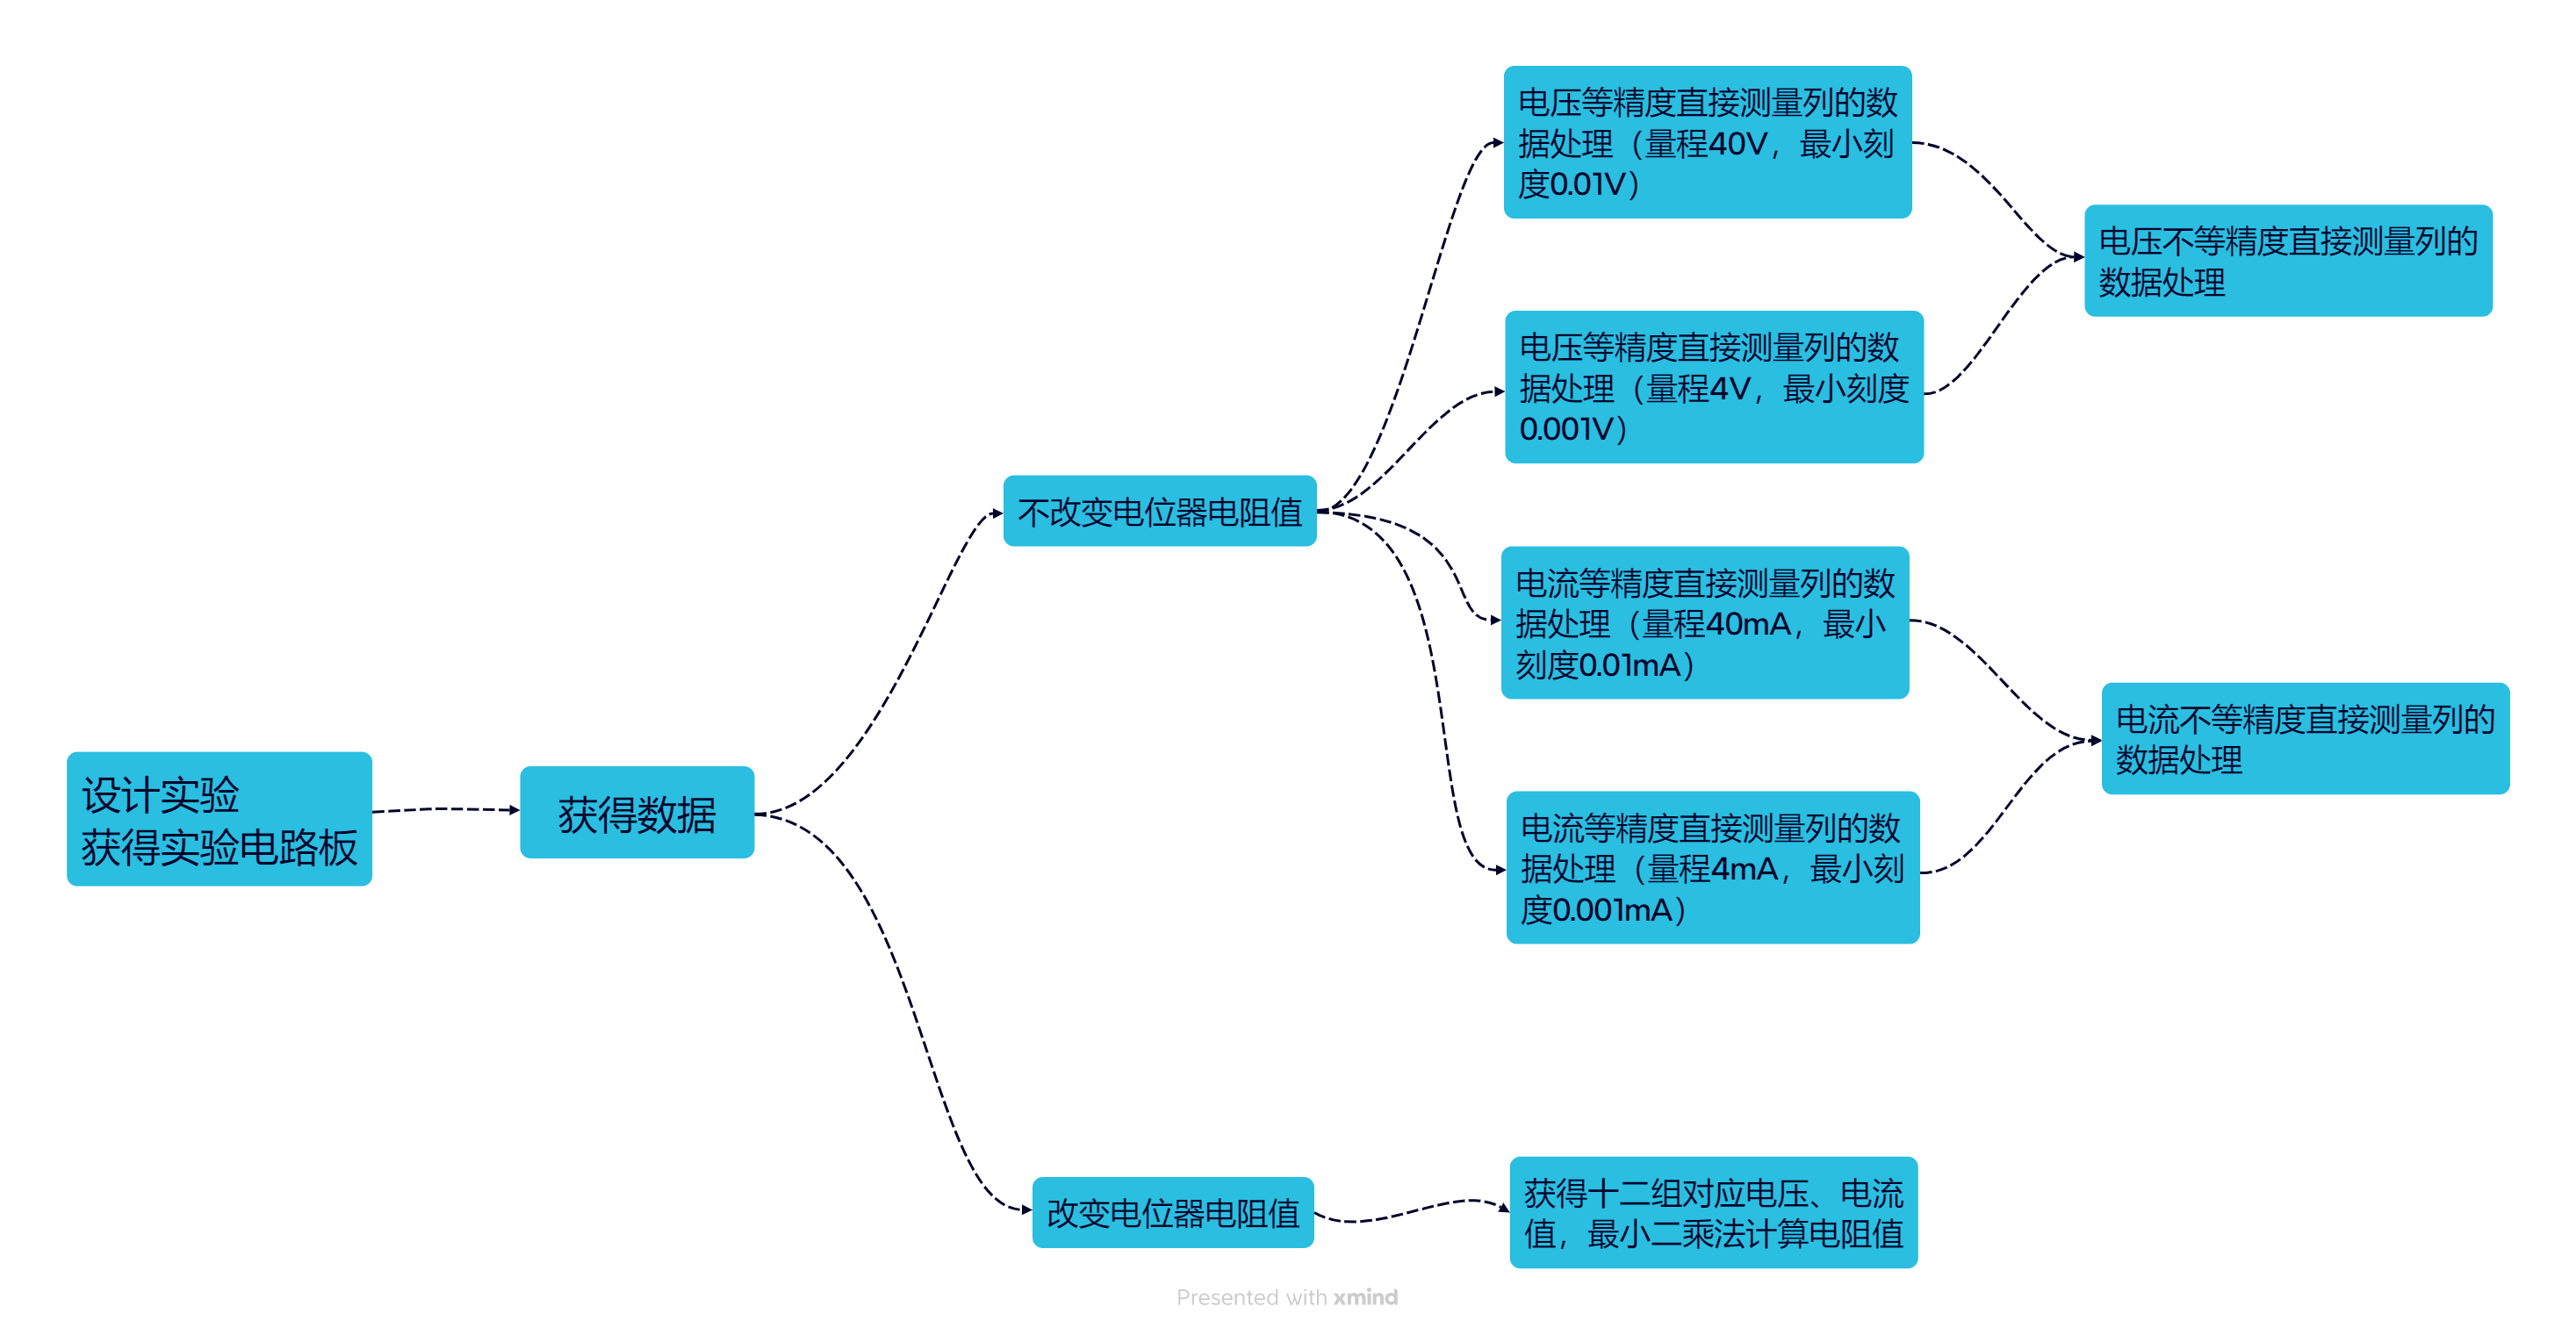
\includegraphics[width=0.8\textwidth]{../截图/获得数据}
		\end{figure}
	\end{frame}
	\subsection{实验设计}
		\begin{frame}{实验设计}  %开始一张幻灯片
			\begin{columns}[c]  %开始进入分栏环境，居中设置
				\column{8cm}  %第一栏（左栏）宽度为8cm
				\text{欧姆定律：}
				\begin{gather*}
					R=\frac{U}{I}
				\end{gather*}	
				\textit{欧姆定律为“伏安法”测电阻的的原理公式。}\\
				\textit{基于此基本公式，设计了右侧的原理电路。}
				\column{3cm}
				\begin{figure}
				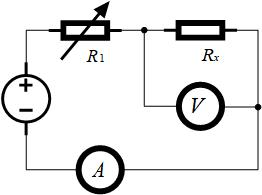
\includegraphics[width=\textwidth]{../截图/电路原理图} 
				\end{figure}
			\end{columns}  %分栏环境结束
			\vspace{30 pt} 
			由于我们在实际电路中采用电流表外接的形式。因此需要在后续数据处理时考虑电压表内阻通过的电流，对实验的影响。
		\end{frame}
		\begin{frame}
			基于实验原理图，设计出实际的原理图，电路板仿真图和电路板实物图。
			\begin{columns}[c]  %开始进入分栏环境，居中设置
				\column{0.35\textwidth}  
				\begin{figure}
					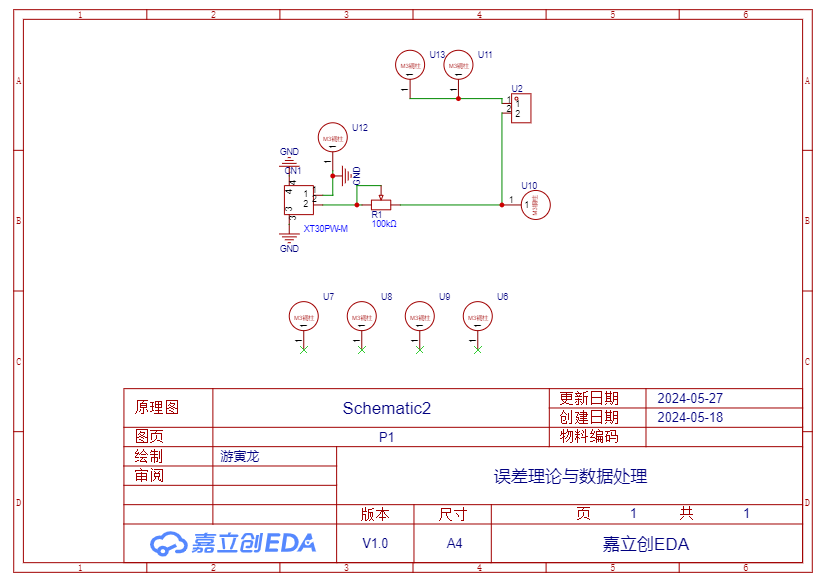
\includegraphics[width=\textwidth]{../截图/电路板原理图} 
				\end{figure}
				\column{0.35\textwidth}
				\begin{figure}
					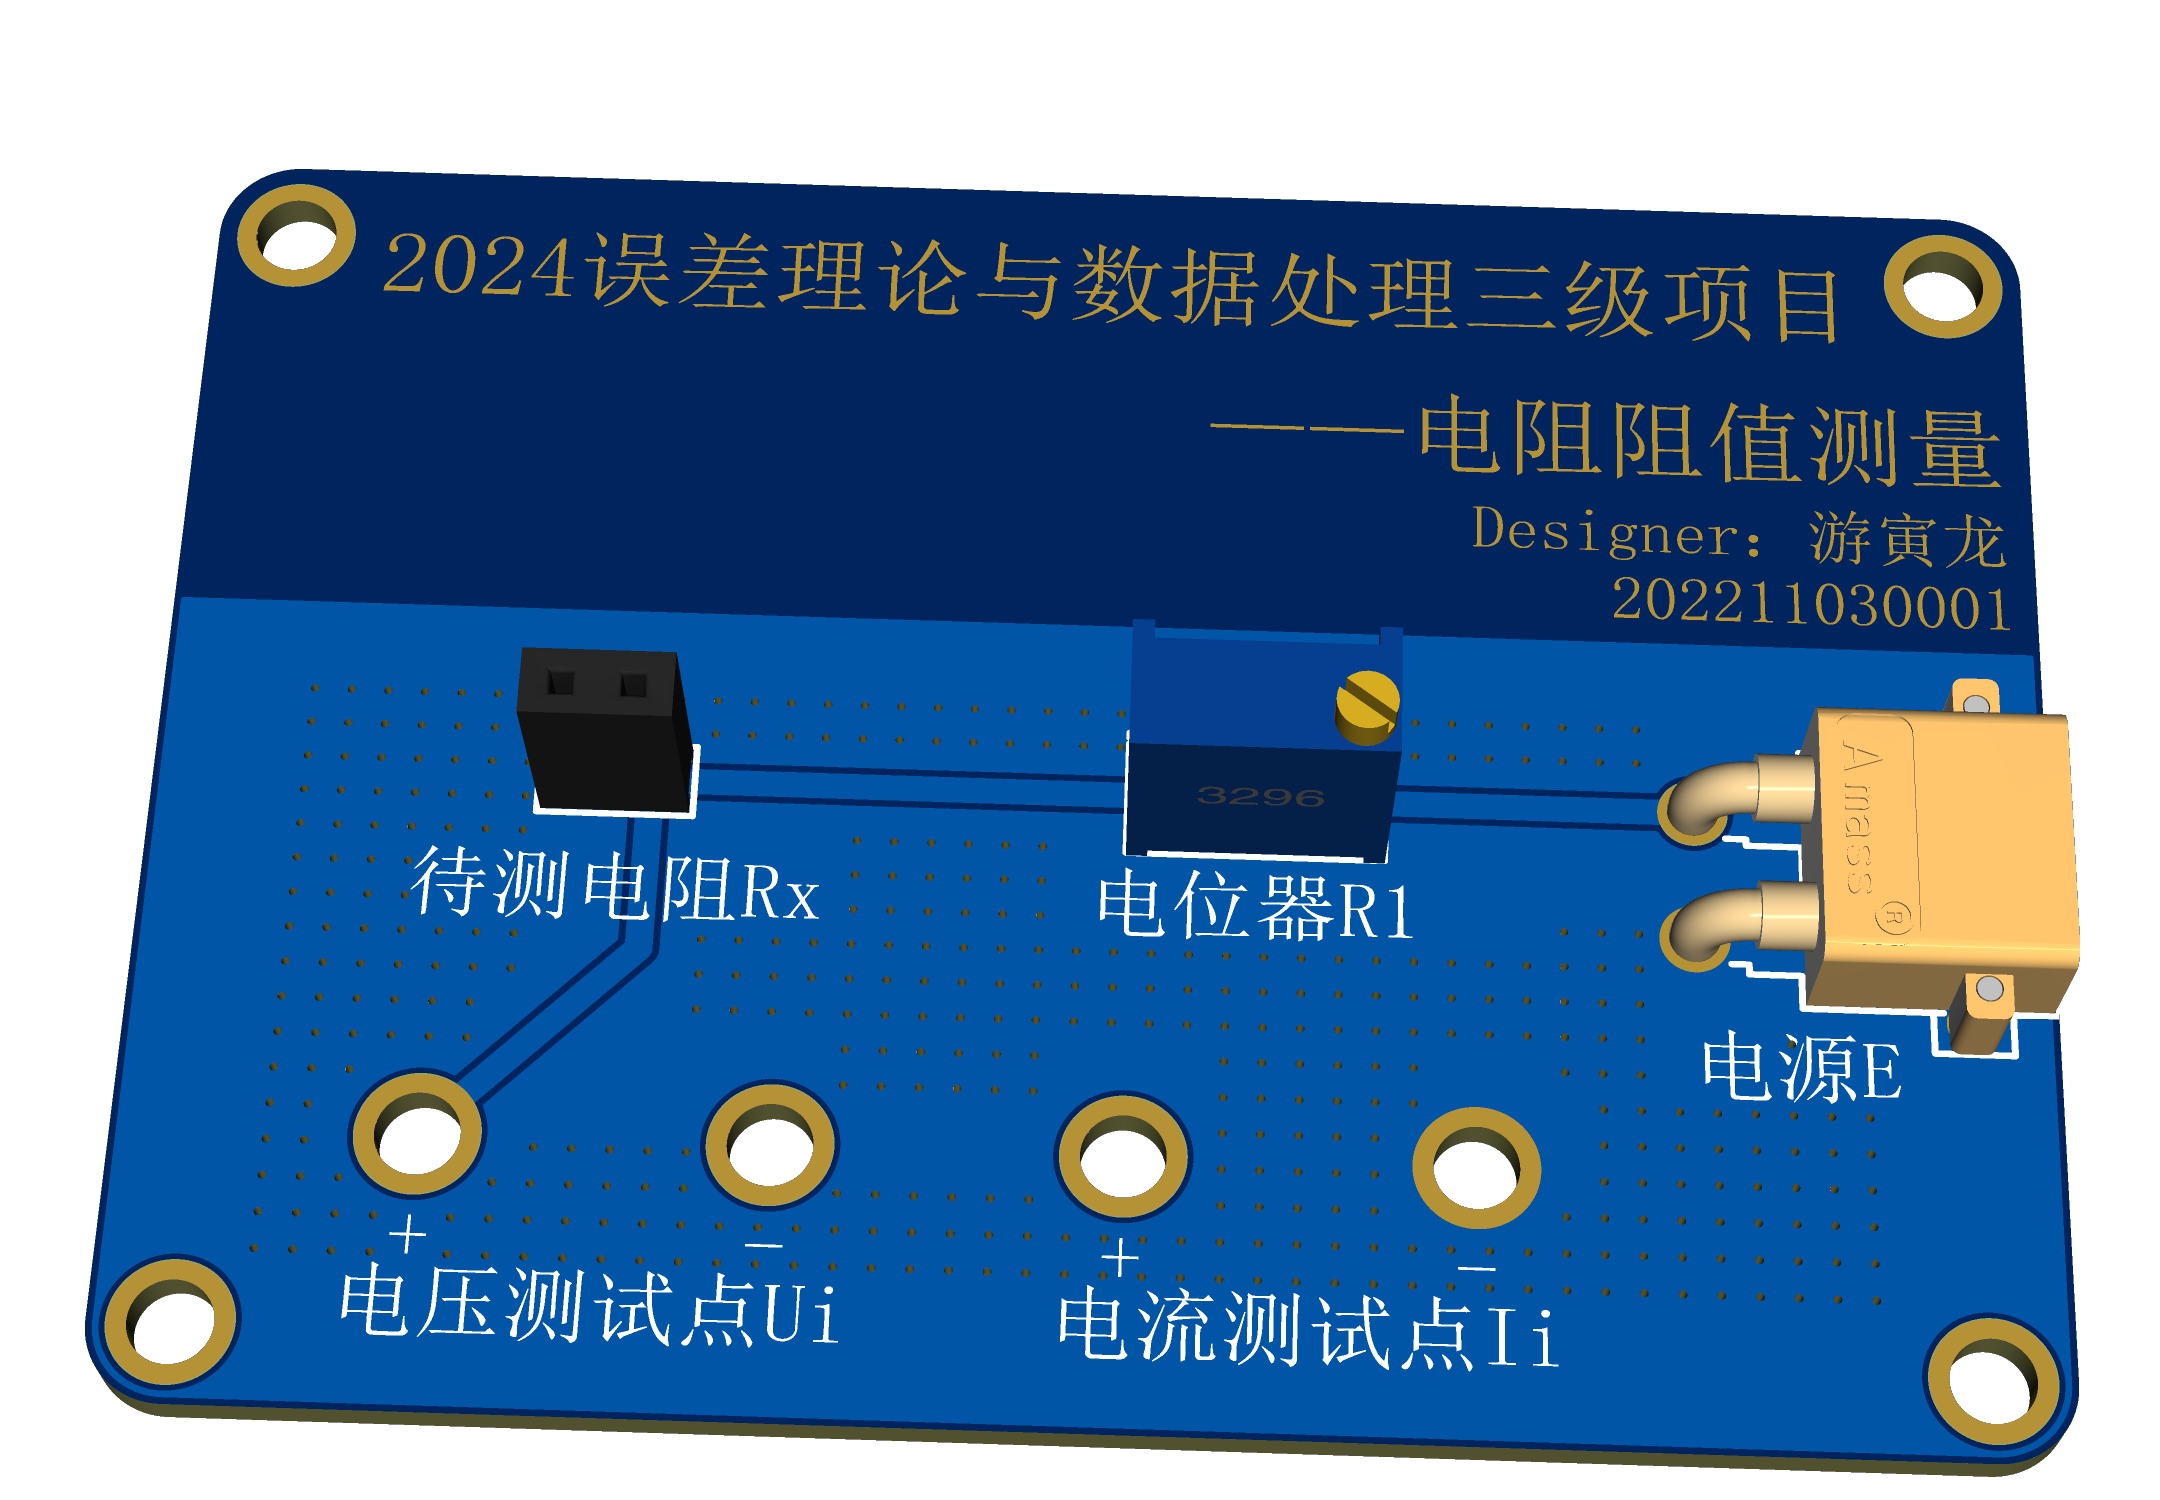
\includegraphics[width=\textwidth]{../截图/电路板3D仿真图} 
				\end{figure}
			\end{columns} 
			\begin{figure}
				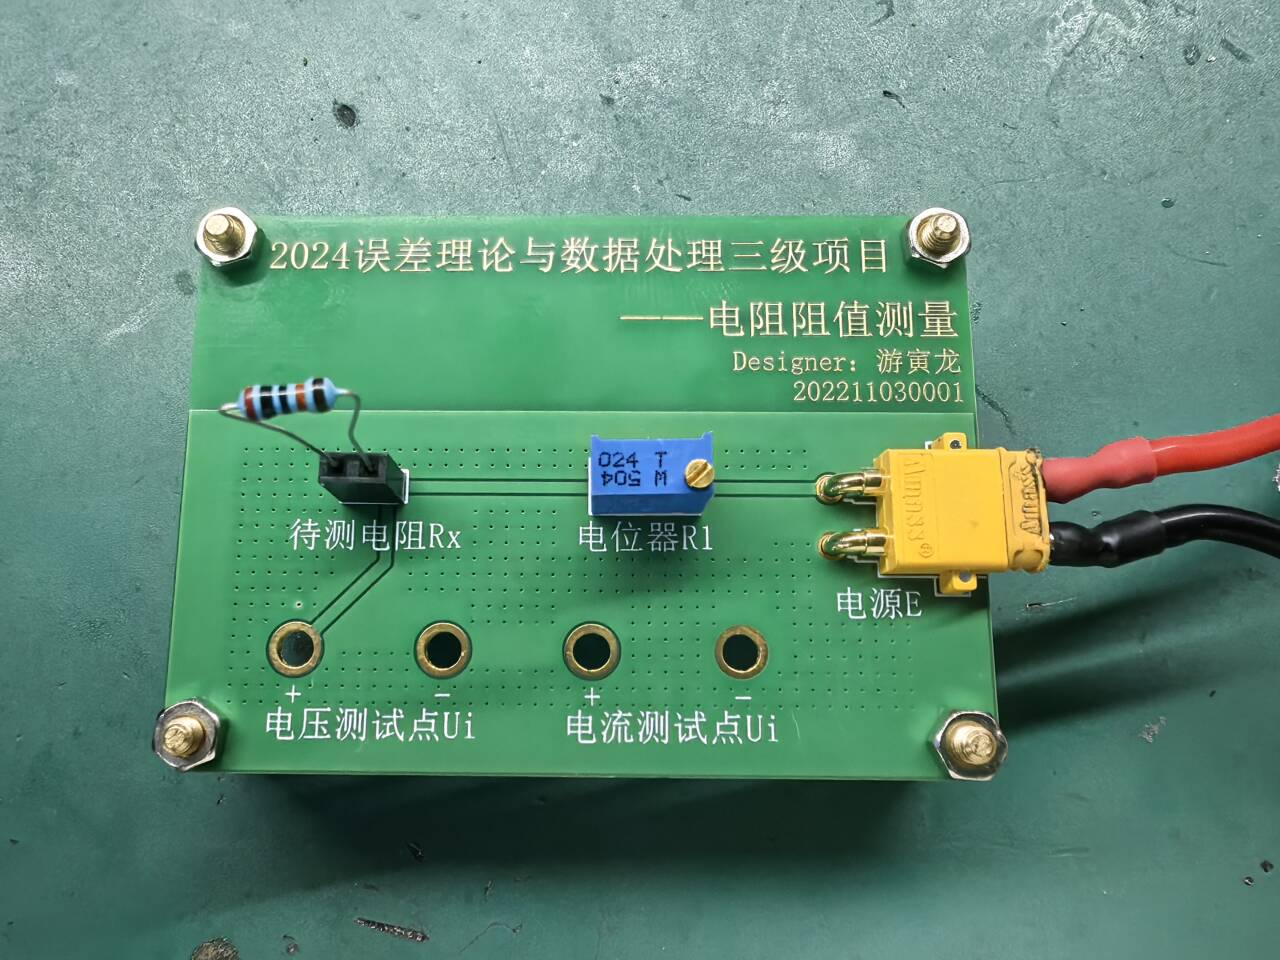
\includegraphics[width=0.35\textwidth]{../截图/电路板实际图} 
			\end{figure}
		\end{frame}
	\subsection{数据测量}
		\begin{frame}{数据测量}
			在实际测量中，使用了两个同样型号（型号：LCSC530+）的万用表进行。
			\begin{columns}[c]  %开始进入分栏环境，居中设置
				\column{0.35\textwidth}  
				\begin{figure}
					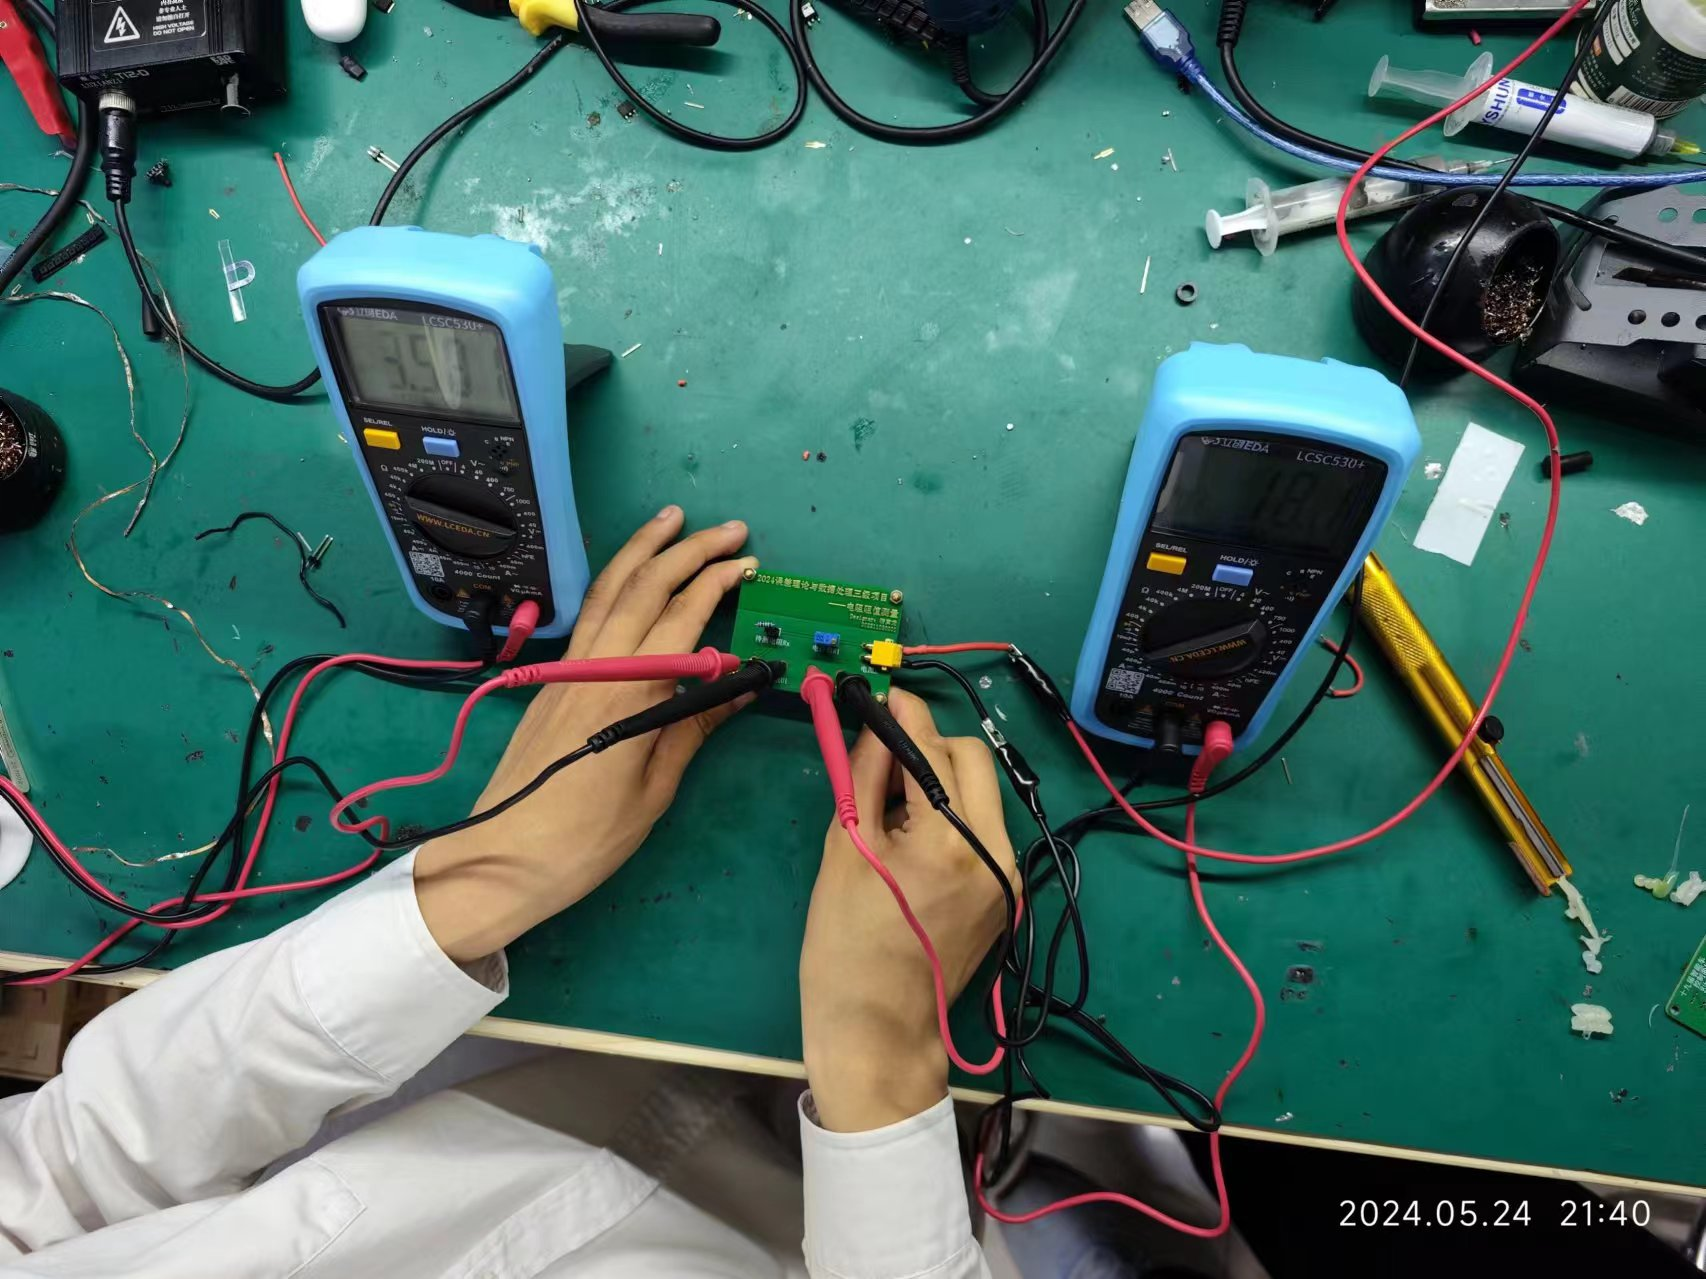
\includegraphics[width=\textwidth]{../截图/实际测量1} 
				\end{figure}
				\column{0.35\textwidth}
				\begin{figure}
					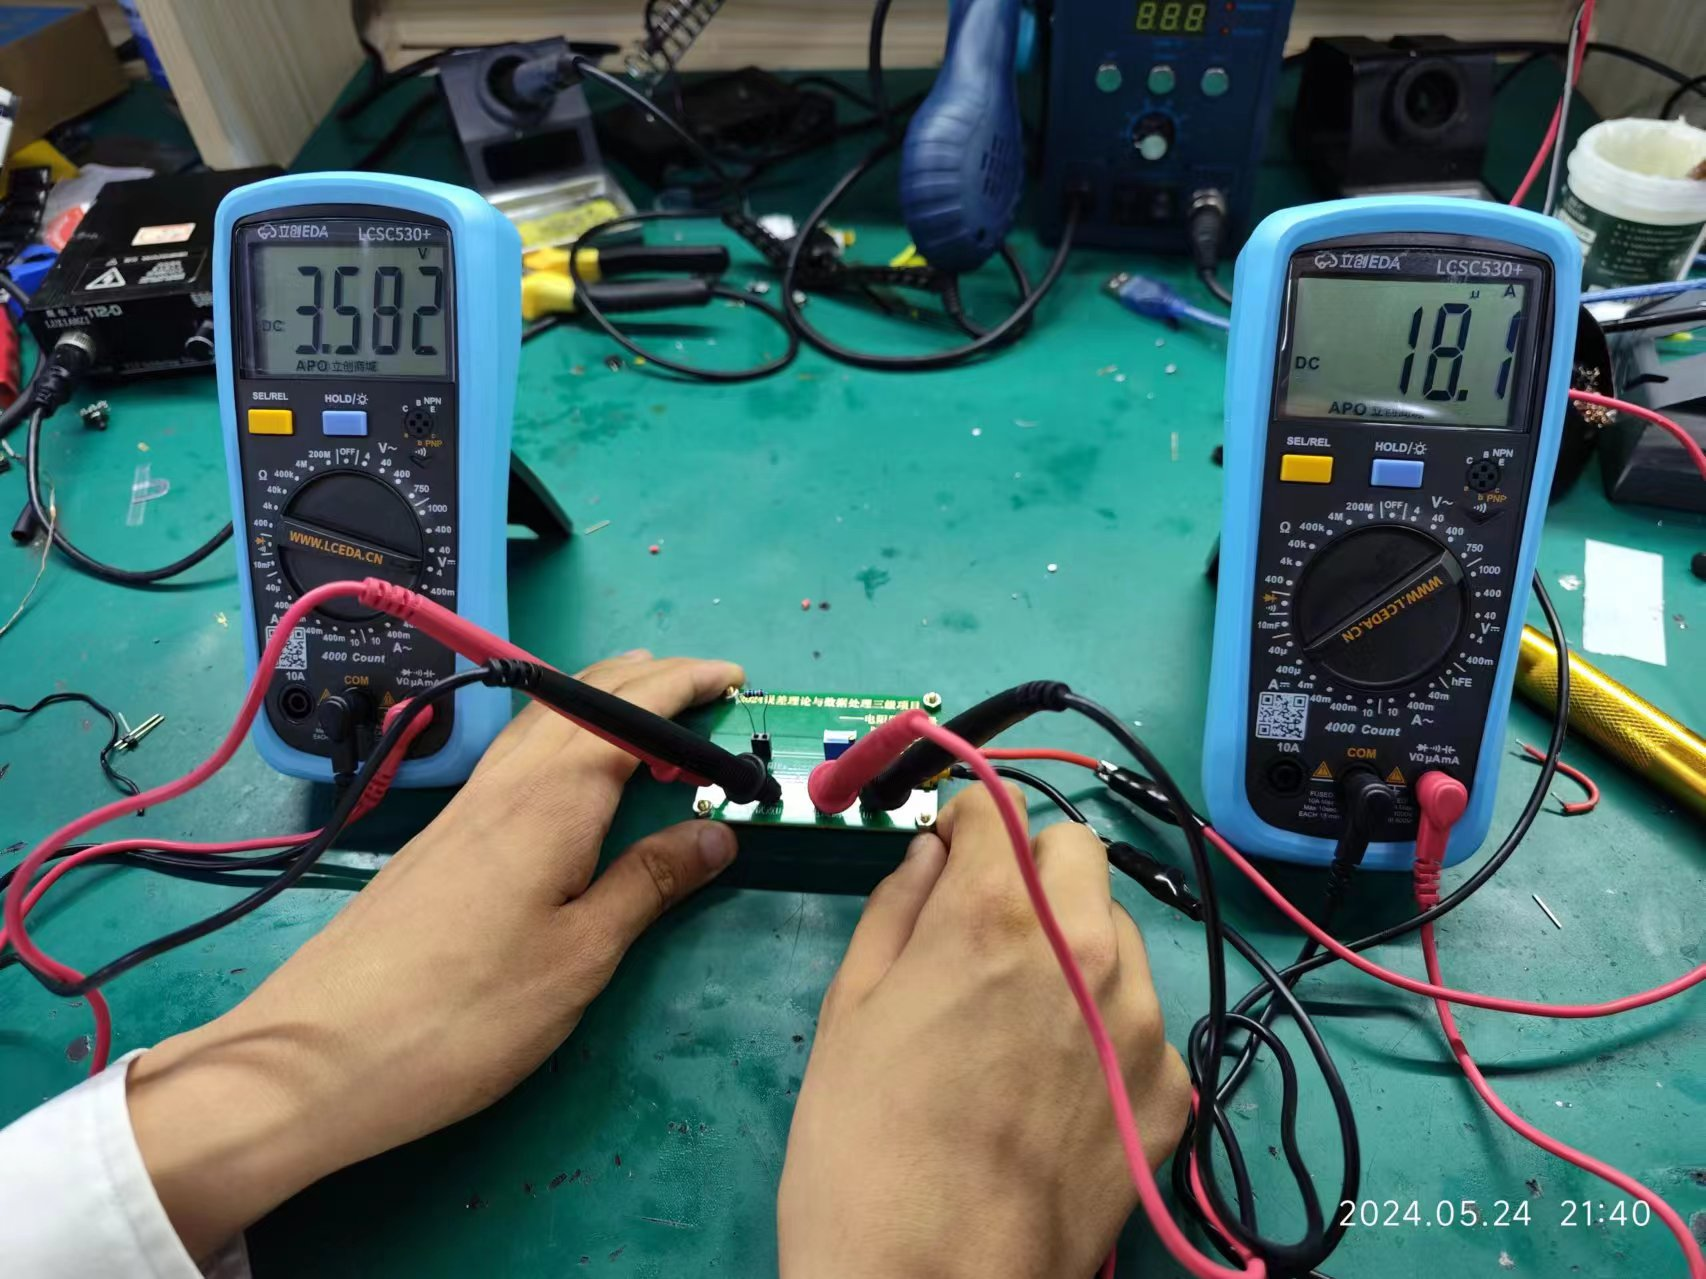
\includegraphics[width=\textwidth]{../截图/实际测量2} 
				\end{figure}
			\end{columns}
			\vspace{15 pt}
			\begin{itemize}
				\item 左侧表作为电压表使用，测量电压
				\item 右侧表作为电流表使用，测量电流
			\end{itemize}
		\end{frame}
		
		\begin{frame}
			测量结果如下所示
			\begin{table}
				\begin{tabular}{c| c| c|| c| c||c|c}%r右对齐，c居中，l左对齐
					\hline
					项目 & \multicolumn{2}{c||}{电压测量}& \multicolumn{2}{c||}{电流测量}& \multicolumn{2}{c}{最小二乘估算}\\
					\hline
					量程 & 40V & 4V &400$\upmu$A&40$\upmu$A& 4V&40$\upmu$A\\
					\hline
					最小分度& 0.01V&0.001V&0.1$\upmu$A&0.01$\upmu$A&0.001V&0.01$\upmu$A\\
					\hline
					\multirow{9}*{测量结果}&3.57&3.578&18.0&18.09&0.530&2.83\\
					\multirow{9}*{}&3.58&3.580&18.1&18.09&0.569&3.01\\
					\multirow{9}*{}&3.58&3.582&18.1&18.09&1.013&5,25\\
					\multirow{9}*{}&3.58&3.580&18.0&18.08&1.822&9.33\\
					\multirow{9}*{}&3.58&3.577&18.1&18.09&1.824&9.36\\
					\multirow{9}*{}&3.57&3.583&18.0&18.09&2.058&10.49\\
					\multirow{9}*{}&&3.586&&18.08&2.557&13.00\\
					\multirow{9}*{}&&3.579&&18.09&2.701&13.73\\
					\multirow{9}*{}&&3.584&&18.08&3.039&15.42\\
					\multirow{9}*{}&&&&&$\cdots$&$\cdots$\\
					\hline
					组数&6&9&6&9&16&16\\
					\hline
				\end{tabular}
			\end{table}
		\end{frame}
\section{处理步骤}
	\begin{frame}{处理步骤}
		等精度处理步骤：
		\begin{columns}[c]  %开始进入分栏环境，居中设置
			\column{0.5\textwidth}
			\begin{enumerate}
				\item 求算术平均值
				\item 求残余误差
				\item 校核算术平均值及其残余误差
				\item 判断系统误差
				\item 求测量列单次测量的标准差
				\item 判断粗大误差
				\item 求算术平均值的标准差
				\item 求算术平均值的极限误差
				\item 写出最后测量结果
			\end{enumerate}
			\column{0.5\textwidth}
			\begin{figure}
				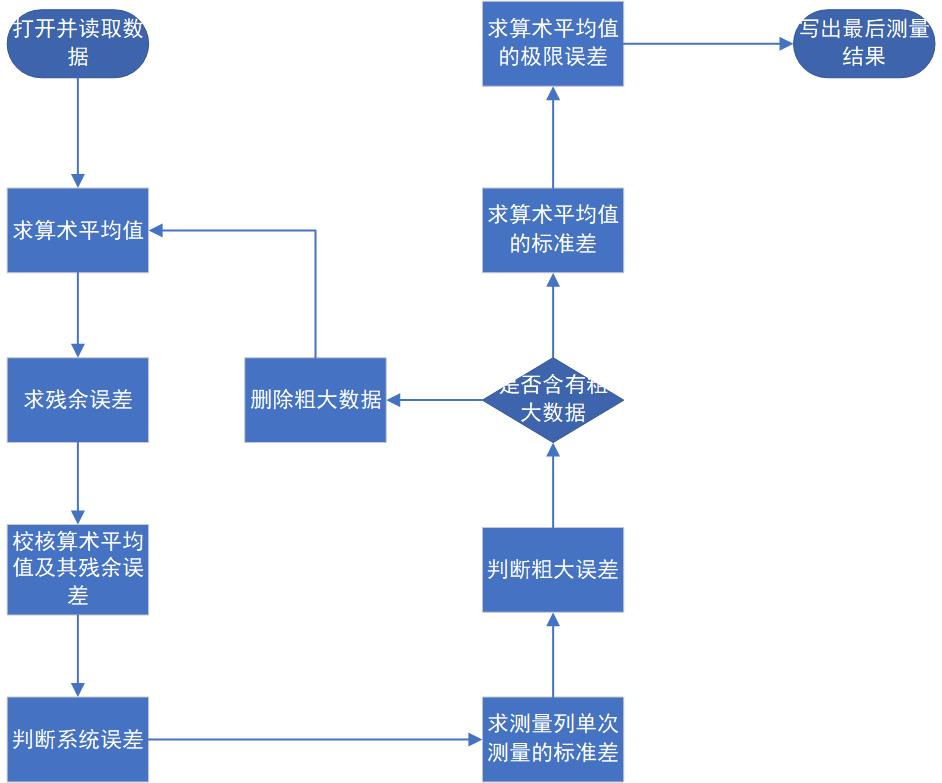
\includegraphics[width=\textwidth]{../截图/等精度流程图} 
			\end{figure}
		\end{columns}
	\end{frame}
	\begin{frame}
		不等精度处理步骤：
		\begin{columns}[c]  %开始进入分栏环境，居中设置
			\column{0.5\textwidth}
			\begin{enumerate}
				\item 求加权算术平均值
				\item 求残余误差
				\item 求加权算术平均值的标准差
				\item 求加权算术平均值的极限误差
				\item 写出最后测量结果
			\end{enumerate}
			\column{0.5\textwidth}
			\begin{figure}
				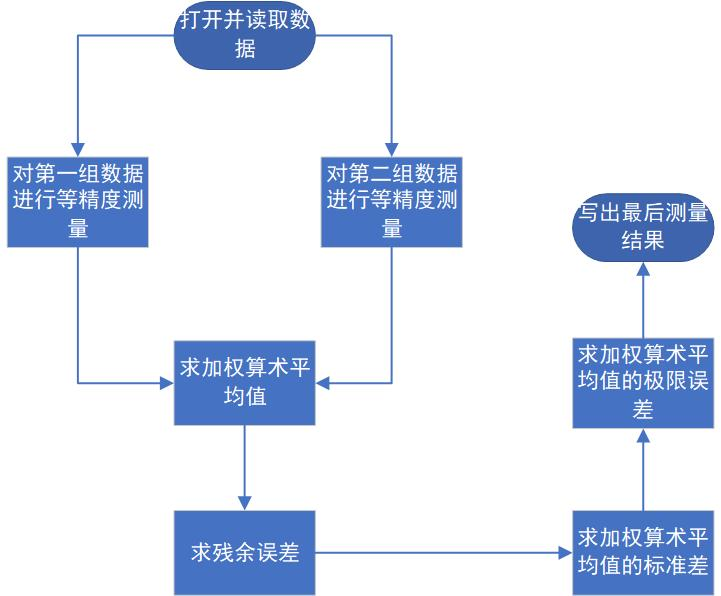
\includegraphics[width=\textwidth]{../截图/不等精度流程图} 
			\end{figure}
		\end{columns}
	\end{frame}
	\begin{frame}
		最小二乘法（矩阵法）处理步骤：
		\begin{columns}[c]  %开始进入分栏环境，居中设置
			\column{0.5\textwidth}
			\begin{enumerate}
				\item 列出误差方程
				\item 列出正规方程
				\item 求解估计量
				\item 计算测量数据的标准差
				\item 计算估计量的标准差
				\item 写出最后估算结果
			\end{enumerate}
			\column{0.45\textwidth}
			\begin{gather*}
				V=L-A\hat{X}
			\end{gather*}
			\begin{gather*}
				C=A^T A
			\end{gather*}
			\begin{gather*}
				\hat{X}=C^{-1}A^TL=(A^TA)^{-1}A^TL
			\end{gather*}
			\begin{gather*}
				\sigma=\sqrt{\frac{V^T V}{n-t}}
			\end{gather*}	
		\end{columns}
	\end{frame}
\section{程序编写}
	\subsection{软件环境}
	\begin{frame}{软件环境}
		\begin{columns}[c]  %开始进入分栏环境，居中设置
			\column{0.45\textwidth}
			数据处理软件：MWorks\\
			\vspace{5pt}
			环境语言：Julia
			\begin{figure}
				
\includegraphics[width=0.5\textwidth]{../截图/MWORKS图标} 
			\end{figure}
			
			\column{0.45\textwidth}
			数据管理软件：Excel\\
			\vspace{5pt}
			环境语言：VBA
			\begin{figure}
				
\includegraphics[width=0.5\textwidth]{../截图/CSV图标} 
			\end{figure}
		\end{columns}
	\end{frame}
	\subsection{完整代码}
	\begin{frame}{完整代码}
		共三个文件:等精度.jl \quad 不等精度.jl \quad 矩阵法最小二乘法.jl\\
		代码量共计380+行（等精度242行；不等精度76行；矩阵法最小二乘法64行）\\
		等精度：
		\begin{columns}[c]  %开始进入分栏环境，居中设置
			\column{0.3\textwidth}
			\begin{figure}
				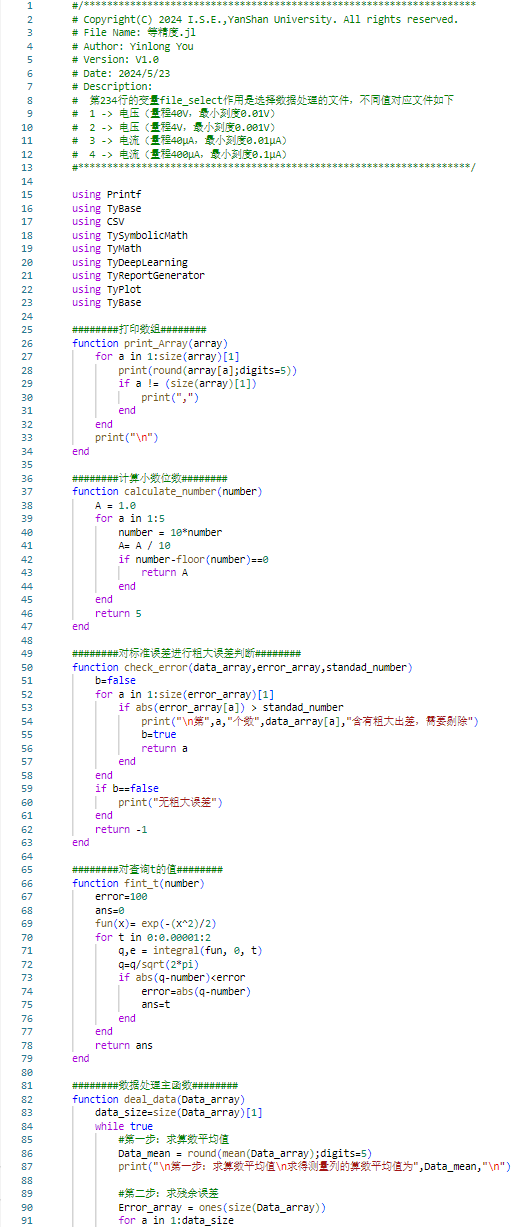
\includegraphics[width=0.5\textwidth]{../截图/等精度处理代码_1} 
			\end{figure}
			\column{0.3\textwidth}
			\begin{figure}
				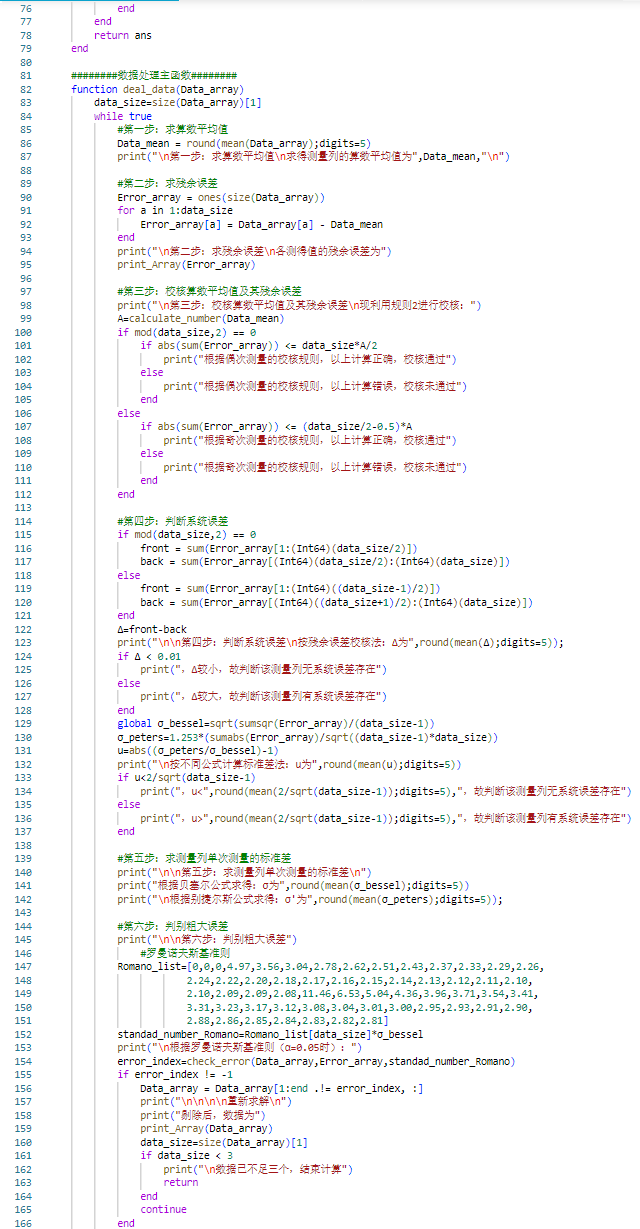
\includegraphics[width=0.5\textwidth]{../截图/等精度处理代码_2} 
			\end{figure}
			\column{0.3\textwidth}
			\begin{figure}
				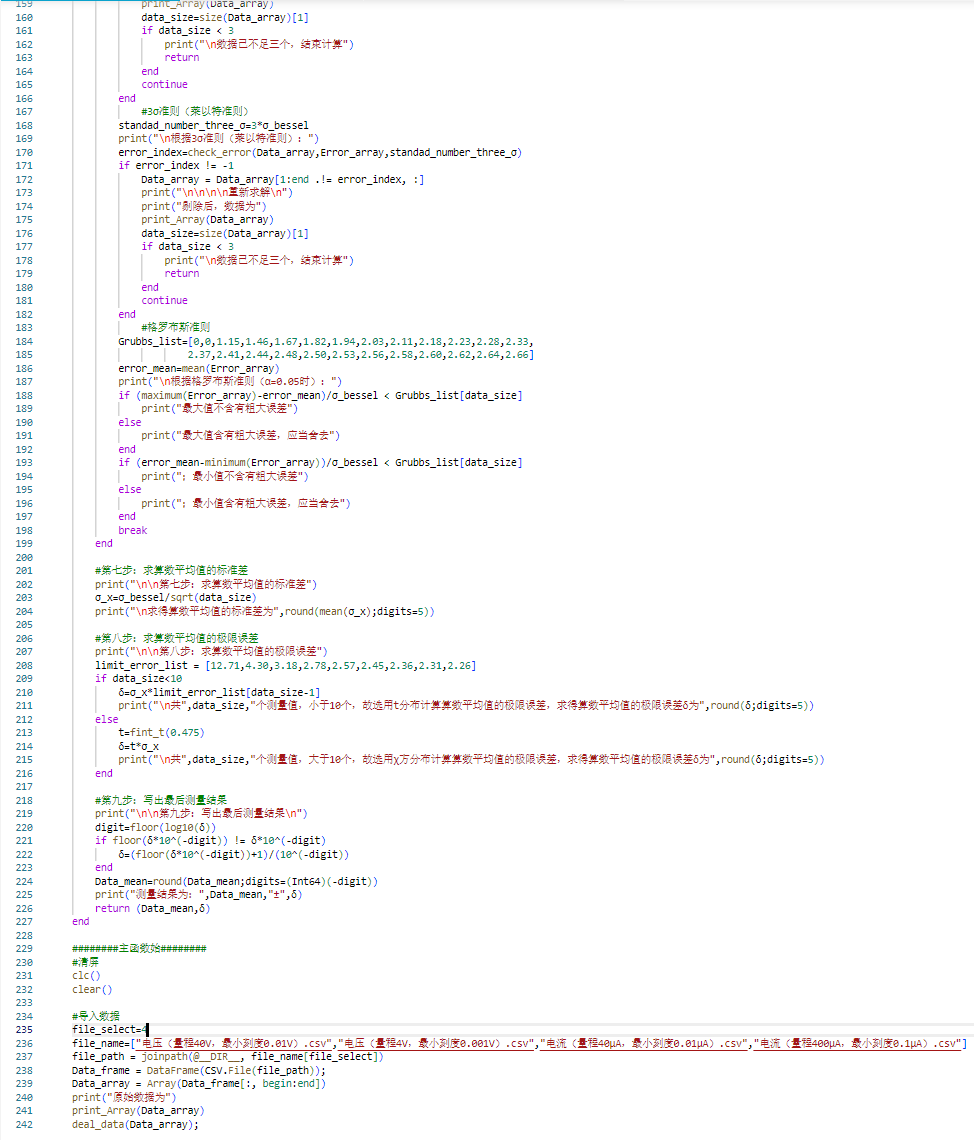
\includegraphics[width=0.5\textwidth]{../截图/等精度处理代码_3} 
			\end{figure}
		\end{columns}
	\end{frame}
	\begin{frame}	
		\begin{columns}[c]  %开始进入分栏环境，居中设置
			\column{0.45\textwidth}
			不等精度：
			\begin{figure}
				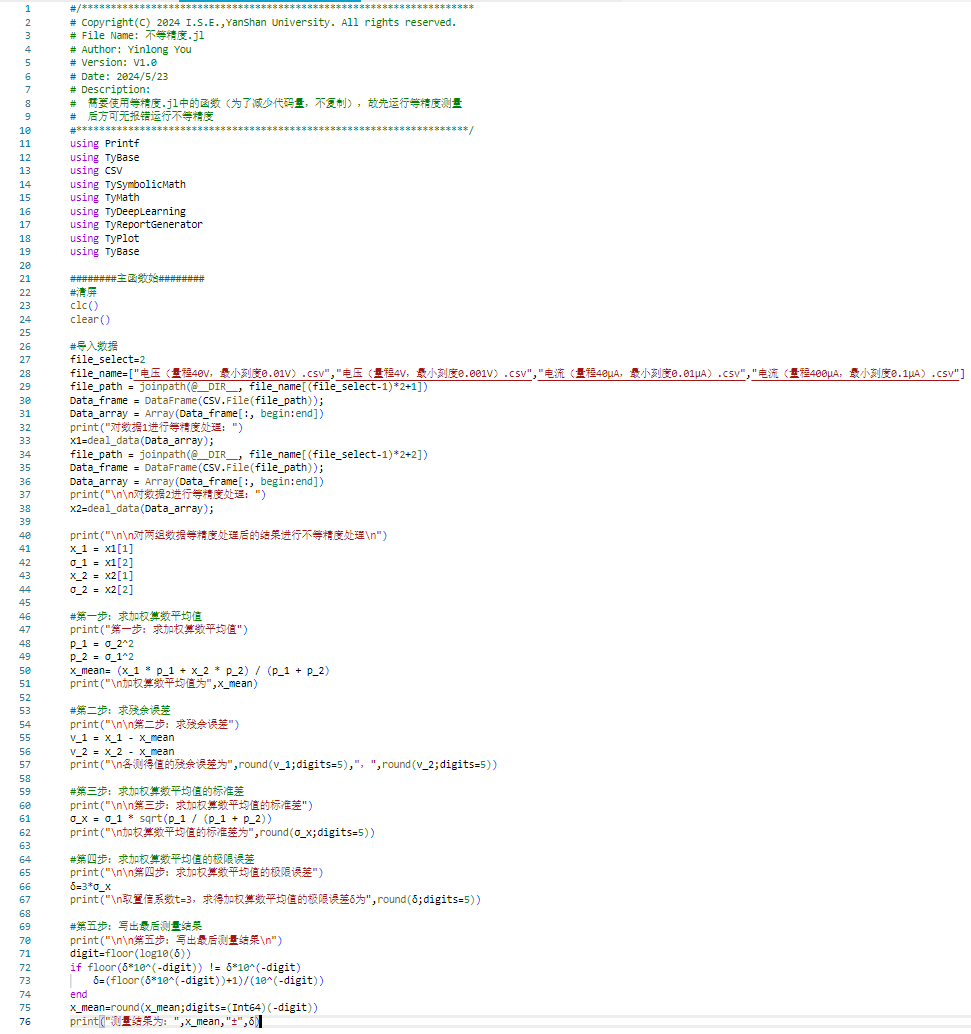
\includegraphics[width=0.9\textwidth]{../截图/不等精度处理代码} 
			\end{figure}
			\column{0.45\textwidth}
			最小二乘法估算（矩阵法）：
			\begin{figure}
				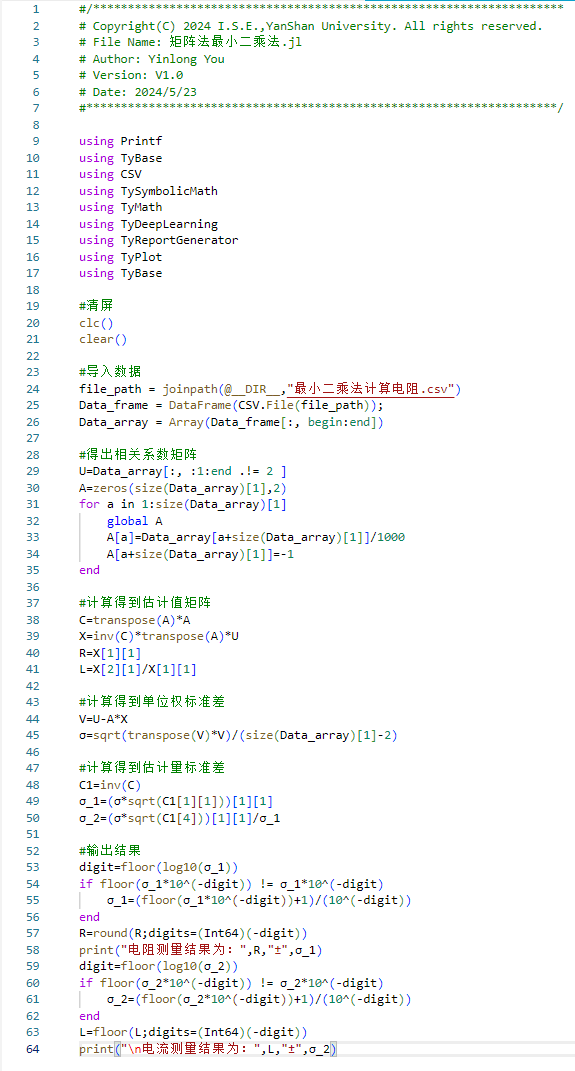
\includegraphics[width=0.5\textwidth]{../截图/最小二乘法回归运算代码} 
			\end{figure}
		\end{columns}
	\end{frame}
\section{结果展示}
	\begin{frame}{结果展示}
		\begin{columns}[c]  %开始进入分栏环境，居中设置
			\column{0.45\textwidth}
			等精度：
			\begin{enumerate}
				\item 求算术平均值
				\item 求残余误差
				\item 校核算术平均值及其残余误差
				\item 判断系统误差(两种方法)
				\item 求测量列单次测量的标准差
				\item 判断粗大误差（三种方法）
				\item 求算术平均值的标准差
				\item 求算术平均值的极限误差
				\item 写出最后测量结果
			\end{enumerate}
			\begin{figure}
			\end{figure}
			\column{0.55\textwidth}
			\begin{figure}
				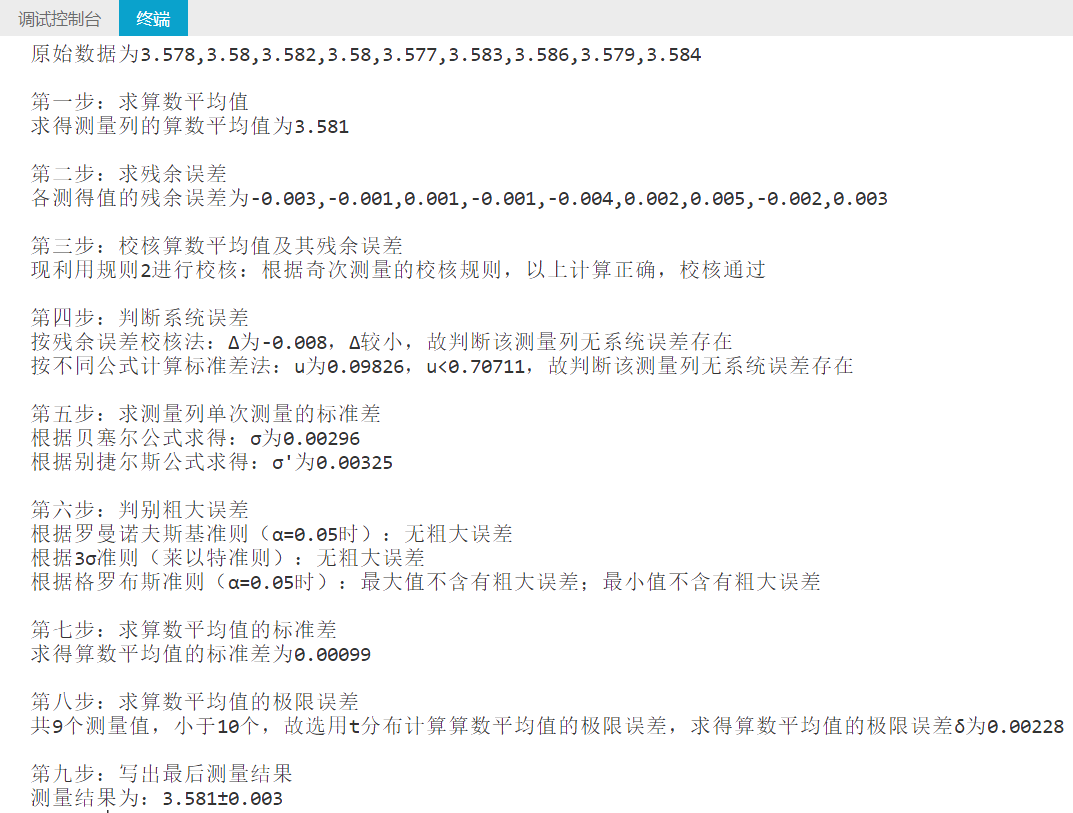
\includegraphics[width=\textwidth]{../截图/电压（量程4V）等精度处理结果} 
			\end{figure}
		\end{columns}
	\end{frame}
	\begin{frame}
		\begin{columns}[c]  %开始进入分栏环境，居中设置
			\column{0.30\textwidth}
			不等精度：
			\begin{enumerate}
				\item 求加权算术平均值
				\item 求残余误差
				\item 求加权算术平均值的标准差
				\item 求加权算术平均值的极限误差
				\item 写出最后测量结果
			\end{enumerate}
			\begin{figure}
			\end{figure}
			\column{0.70\textwidth}
			\begin{columns}[c]
				\column{0.5\textwidth}
				\begin{figure}
					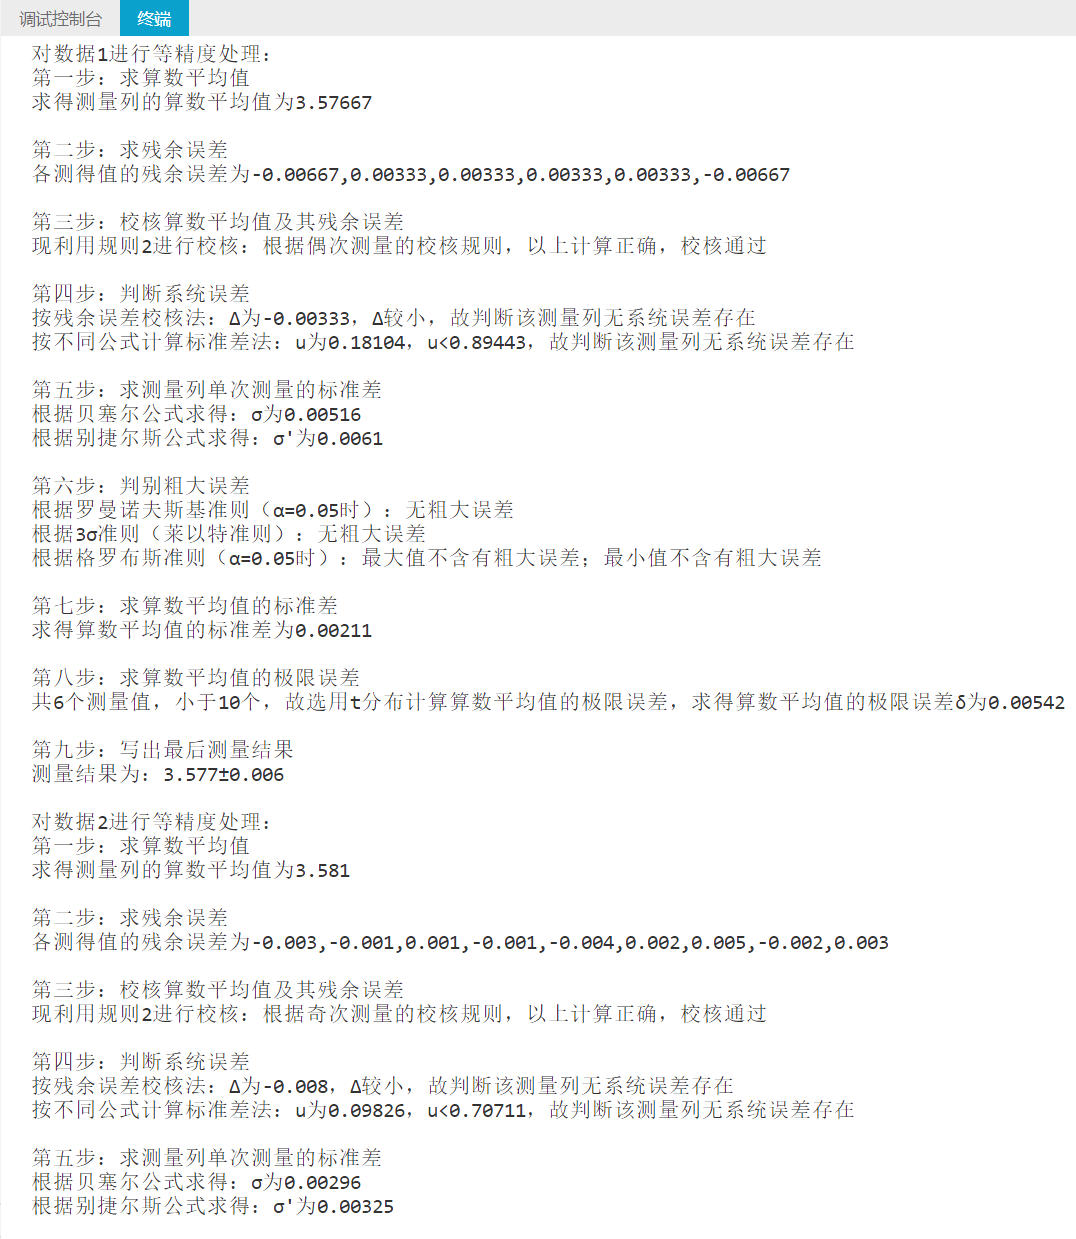
\includegraphics[width=\textwidth]{../截图/电压不等精度处理结果_1} 
				\end{figure}
				\column{0.5\textwidth}
				\begin{figure}
					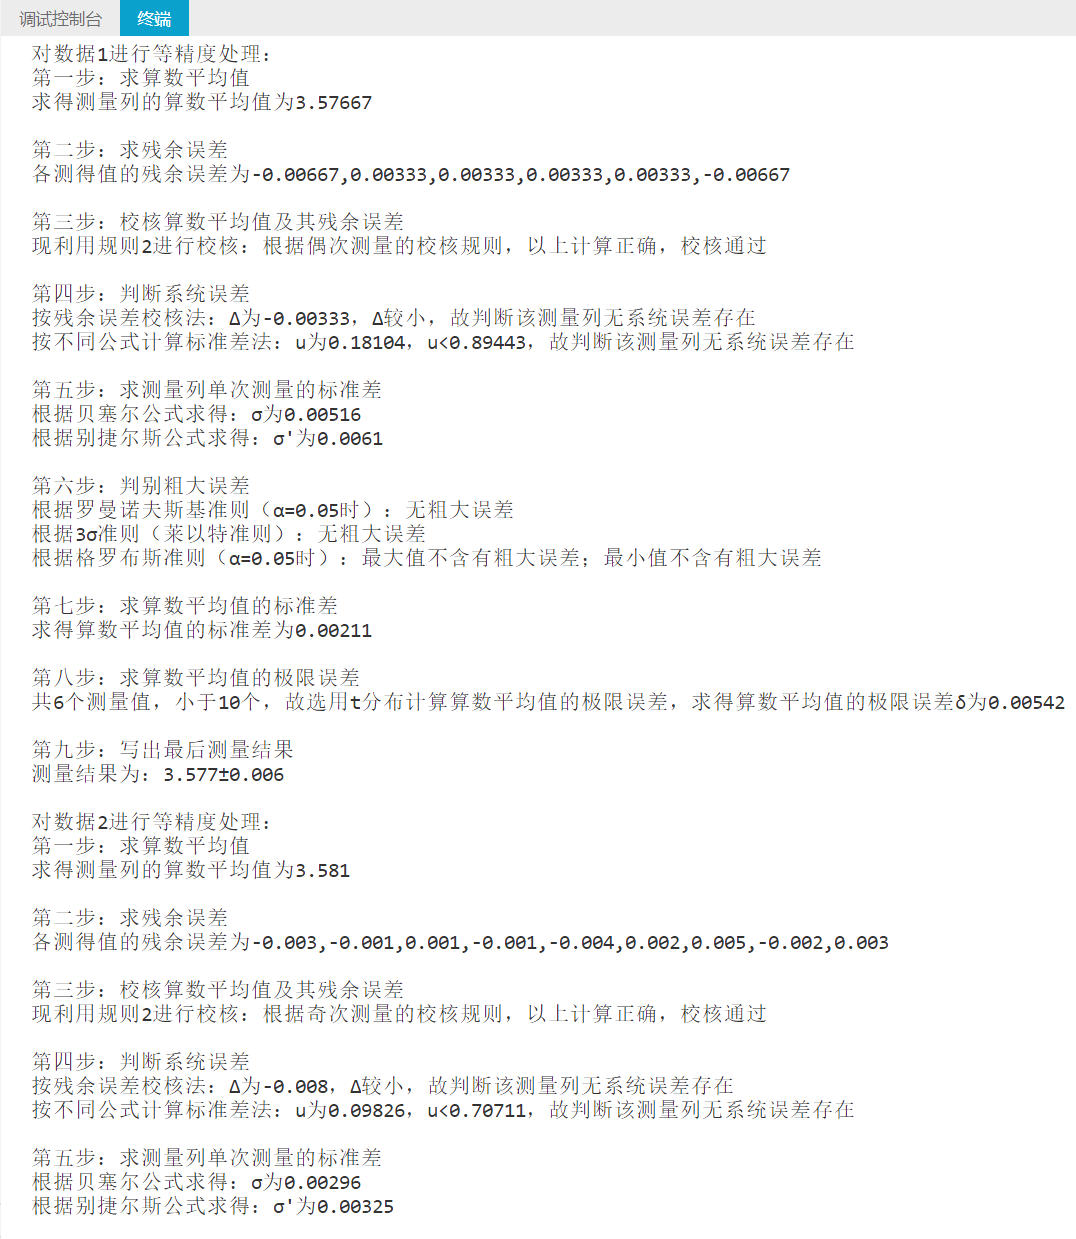
\includegraphics[width=\textwidth]{../截图/电压不等精度处理结果_1} 
				\end{figure}
			\end{columns}
		\end{columns}
	\end{frame}
	
	\begin{frame}
		\begin{columns}[c]
			\column{0.60\textwidth}
			最小二乘法（矩阵法）估算：
			\begin{enumerate}
				\item 列出误差方程
				\item 列出正规方程
				\item 求解估计量
				\item 计算测量数据的标准差
				\item 计算估计量的标准差
				\item 写出最后估算结果
			\end{enumerate}
			电阻色环：红黑黑橙棕\\
			阻值：$200$k$\Omega \pm 1\%=200$k$\Omega \pm 2$k$\Omega$
			\column{0.3\textwidth}
			\begin{figure}
				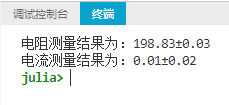
\includegraphics[width=\textwidth]{../截图/最小二乘法回归运算结果} 
			\end{figure}
			\begin{figure}
				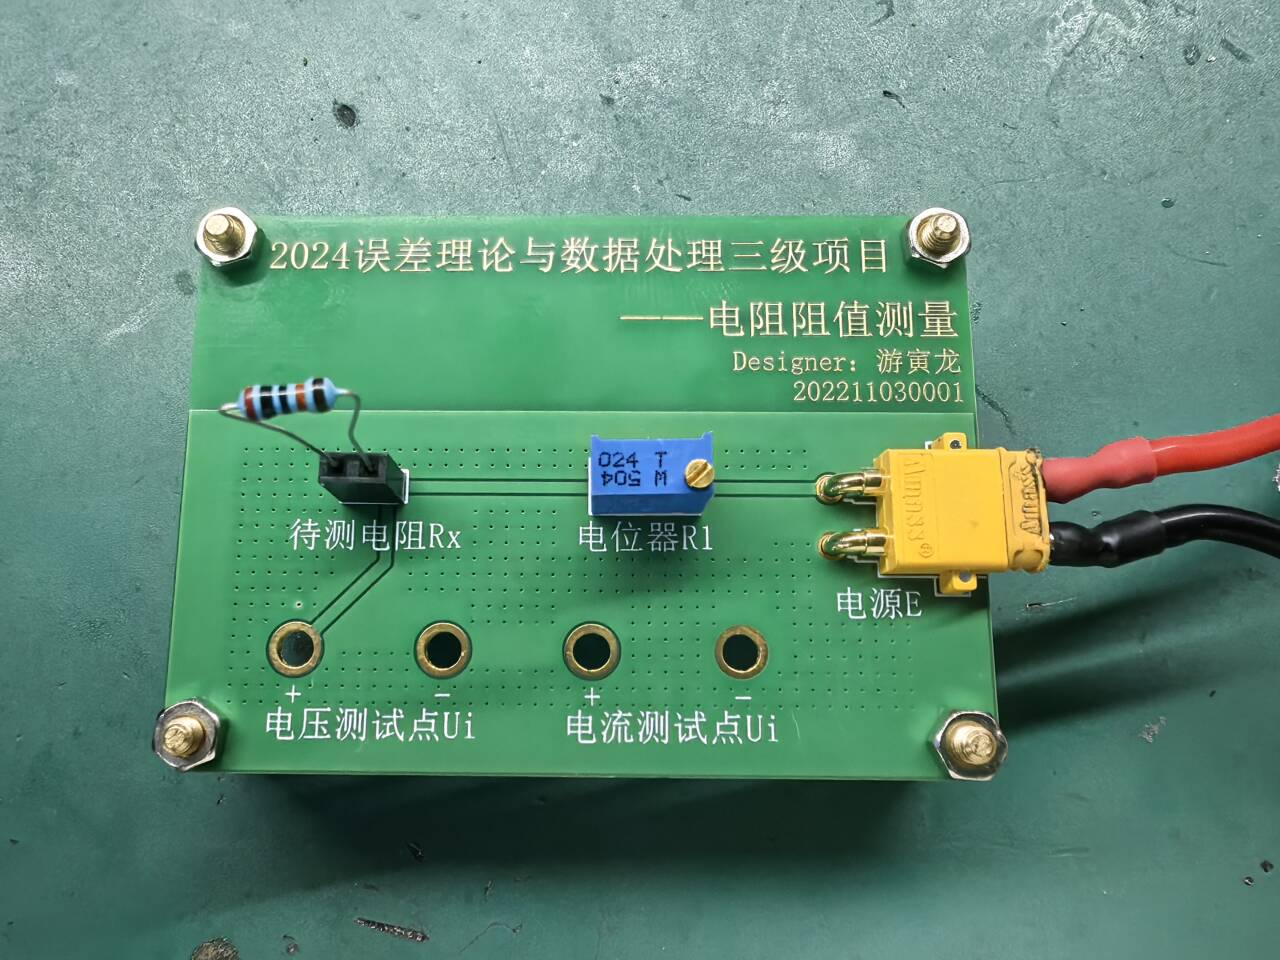
\includegraphics[width=\textwidth]{../截图/电路板实际图} 
			\end{figure}
		\end{columns}
	\end{frame}
	
\section{项目亮点}
	\begin{frame}{实验亮点}
		\begin{block}{实验完整性}
			具有完整的流程，从设计实验、制作实验用具、实践测量、数据处理、数据验证，完全的覆盖了一个实验的所有基本步骤。
		\end{block}
		\begin{block}{软件使用}
			除MWORKS和Excel以外，还用到了以下几个软件。\\
			论文和PPT使用\LaTeXe 编译生成，在公式和格式方面具有更优良的表现。\\
			电路图和流程图使用visio和mwind绘制，在图像表达方面具有更好的便捷性。\\
			
		\end{block}
	\end{frame}
	\begin{frame}{代码亮点}
		\begin{block}{90$\%$原创代码}
			由于MWOKRS网上资源较少（只有官方文档和少部分官方资料）且与MATLAB不尽相同，因此没有任何前人经验。\\
			非原创部分：文件申明注释（30行）引用自反馈三级项目要求；文件导入（12行）引用自官方例程。
		\end{block}
		\begin{block}{生成结果自动化}
			对于任意测量列的数据处理，程序能根据测量次数和组数自动生成完整的等精度和不等精度的全部数据处理。\\
			等精度数据处理中，可以在算出粗大误差后，自动剔除粗大误差，若剩余数据个数$n'>3$，则从第一步开始重新运算。
		\end{block}
	\end{frame}
	\begin{frame}
		\begin{block}{多种方法校验}
			在等精度数据处理中:\\
			系统误差判断使用了残余误差校核法，不同公式计算标准差比较法两种方法。\\
			粗大误差判断使用了莱以特准则、罗曼诺夫斯基准则和格罗布斯准则三种方法。\\
			有效的降低了出错的可能性。
		\end{block}
		\begin{block}{封装等精度数据处理}
			将等精度数据处理的代码封装成函数，利用Julia语言可以跨文件编译的特性，直接在不等精度数据处理中使用。使得代码进一步精炼，自动化程度更高。
		\end{block}
	\end{frame}
	\begin{frame}
		\begin{block}{置信系数的取法}
			根据数据处理的特点，程序自动改变置信系数的取值方法：\\
			等精度数据处理，个数$n<10$时采用学生氏分布；反之则采用正态分布（正态分布使用积分反解方法，夹逼求出高精度的取值，精确到小数点后4位）。\\
			不等精度数据处理，直接采用$t_\alpha=3$进行计算
		\end{block}
		\begin{block}{多处算法实现}
			在校核算数平均值及其残余误差步骤中，规则二要求得到实际求得的算术平均值$\bar{x}$末位数的一个单位$A$。\\
			在极限误差保留一位有效值后，需要将算术平均值末尾数的单位大小和其统一。\\
			对粗大误差舍弃后的重新重头计算。\\
			MWORKS没有都直接可采用的函数，因此需要算法来解决这个问题。\\
		\end{block}
	\end{frame}
\section{总结}
	\begin{frame}{总结}
		在本次实验中，我们组自设实验方案、测量数据。通过误差理论与数据处理的相关手段，对测得电压和电流进行了统计分析，并使用最小二乘法作出了对电阻值的估计。
	\end{frame}
\end{document}